\chapter{脑电图和脑磁图预处理参考}
\label{ch:12}


在本章中,我们将描述所有 SPM/MEEG 预处理和显示功能的功能和语法。
这将是本手册中对这些功能最详细的描述。
我们的目标是提供一个全面的说明,如何使用该软件对脑磁图和脑电图数据进行预处理,直到可以使用某种源重建技术或对脑磁图和脑电图通道数据进行统计分析。

这些功能可以通过 Matlab 命令行和脚本调用,也可以通过批处理输入系统调用。
批处理输入系统设计用于对数据(例如来自多个受试者的数据)进行重复性分析。
一旦用户熟悉了他们分析所需的批处理工具,就很容易通过批处理依赖项将这些工具链接起来,并将它们作为一个流程运行。
批处理工具的使用原则在第 48 章中进行了描述。
命令行功能非常适合编写脚本,或者使用 SPM 的历史记录到脚本功能来自动生成脚本。

对于脚本,我们遵循为每个函数只提供一个输入参数的概念。
这个输入参数通常是一个包含所有输入参数字段的结构(struct)。
这种方法的优点是输入不需要遵循特定的参数顺序。
对于某些参数,可以提供默认值。
当缺少必要参数时,会导致错误。

下面我们将描述批处理工具中可用的参数以及对应的低级 SPM 函数的名称。
这些函数从脚本调用的接口在函数头部中进行了描述。


我们将详细介绍数据转换过程、SPM 中脑磁图和脑电图格式的具体细节、如何正确输入关于通道的附加信息、如何从 SPM 调用 FieldTrip 函数、所有方法和函数的完整参考、如何使用显示功能,最后是如何编写脚本和批处理预处理步骤。


\section{数据转换}

任何分析的第一步是将数据从其原始的、依赖于机器的格式转换为基于 Matlab 的通用 SPM 格式。
该格式将数据存储在 *.dat 文件中,并将所有其他信息存储在 *.mat 文件中。
*.mat 文件包含数据结构 D,而 *.dat 文件是脑电图和脑磁图数据。
SPM 的数据转换功能基于 ‘fileio’ 工具箱,该工具箱在 SPM、FieldTrip 和 EEGLAB 工具箱之间共享,并由这些工具箱的用户共同开发。
目前支持大多数常见的脑电图和脑磁图数据格式。
在某些情况下,可能需要安装额外的 Matlab 工具箱。
这种情况下,会显示错误信息,并提供下载适当工具箱的链接。
如果您的数据格式未被 ‘fileio’ 识别,您可以扩展 ‘fileio’ 工具箱,并将您的代码贡献给我们。
详情请参阅 ‘fileio’ 页面。
 
在脑磁图和脑电图图形用户界面的 Convert 下拉菜单中选择 Convert 后,系统会询问您(‘定义设置?’)是否要为转换定义一些设置,还是选择‘直接读取’。
后者选项被引入以便简单方便地进行数据转换而无需任何额外的询问。
生成的 SPM 脑磁图和脑电图数据文件可以使用 SPM 的审查工具进行探索,以确定未来适合的转换参数。
如果选择‘直接读取’选项,SPM 会尝试在保留尽可能多数据的情况下转换整个数据集。
另一个选项‘是’会打开批处理工具进行转换。
 
无论选择哪种方式,您都需要选择要转换的文件。
一般来说,如果数据集由多个文件组成,应选择包含数据的文件(通常是最大的数据文件)。
SPM 通常可以自动识别数据格式并应用合适的转换程序。
然而,在某些情况下,数据文件中没有足够的信息供 SPM 识别格式。
这种情况通常发生在扩展名不明确的文件(例如 *.dat、*.bin、*.eeg 等)上。
在这种情况下,应选择头文件而不是数据文件进行转换,如果头文件被识别,SPM 将自动定位数据文件。
在某些罕见情况下,自动识别是不可能的,或者对于同一格式有多种可用的低级读取器。
在这些情况下,可以通过批处理工具或脚本强制 SPM 使用特定的低级读取器(见下文)。
 
转换批处理中的其他选项如下:
 
 
读取模式 - 文件可以作为连续数据或时间段数据读取。
在连续模式下,可以读取整个文件或一个连续的时间窗口。
在时间段模式下,应定义试验(见下文的‘时间段’)。
在转换时定义试验的优点是,只转换原始数据中所需的子集。
这在感兴趣的试验仅占整个记录的一小部分时非常有用(例如,睡眠期间记录的一些事件)。
请注意,有些数据集一开始并不包含连续数据。
这些数据集通常应使用‘时间段’选项进行转换。
此外,还可以只转换头文件而不转换数据。
如果感兴趣的信息在头文件中(例如传感器位置),这种方法会很有用。
 
 
通道选择 - 可以选择一个通道子集。
有几种定义该子集的方法,可以结合使用:按通道类型、按名称或使用包含通道标签列表的 *.mat 文件。
请注意,通道选择分支在许多批处理工具中都有提供,其功能在所有地方都是相同的。
 
 
输出文件名 - 指定输出数据集的名称。
请注意,在这里可以任意命名输出文件名,而在其他预处理工具中,用户只能定义附加到现有名称的前缀(此限制可以通过使用‘复制’工具来绕过)。
默认情况下,SPM 会在原始数据文件名中添加‘spmeeg\_’前缀。


事件填充 - 通常在转换时划分时间段时,只包括试验中的事件。
此选项使得可以在指定时间窗口内,也包括发生在时间段之前和之后的事件。


块大小 - 这是用于读取大文件时内部使用的块的大小。
通常不需要修改,除非您使用的是内存有限的旧系统。


检查试验边界 - 如果从原始数据文件明显看出数据不是连续的,SPM 通常不会将其读取为连续数据,并会给出错误提示。
在一些罕见的情况下,可能需要绕过此限制(例如,如果真正的连续数据以块(伪时间段)的形式存储,且 SPM 无法自动识别时)。


保存原始头文件 - 通用的 fileio 接口无法传递所有特定格式可用的头文件字段。
有时,这些缺少的头文件字段对于某些特定功能是必要的,此选项允许将完整的原始头文件作为转换后头文件的一个子字段保留。
一个特别有用的场景是处理 CTF 脑磁图系统中的连续头部定位数据,该系统需要一些来自原始头文件的信息来解释数据。


输入数据格式 - 此选项允许强制使用特定的低级读取器来转换数据。
通常不需要这样做。
高级用户可以在 ft\_read\_header 函数的代码中找到该字段的可能值。


\section{转换任意数据}

如果您的数据不属于任何标准格式,而只是作为 ASCII 文件、Excel 文件或 Matlab 工作区中的变量可用,那么您有两种选择,取决于您是否愿意使用 Matlab 脚本,或只想使用图形用户界面。

SPM 中的‘准备’界面有一个选项,可以将 Matlab 工作区中的变量转换为 SPM 格式。
只需回答几个问题以确定数据的维度和时间轴。
其他信息(例如通道标签)可以通过 SPM 审查工具提供。

如果您愿意编写一个简单的 Matlab 脚本,最直接的方法是创建一个简单的 FieldTrip 原始数据结构(Matlab 结构体),然后使用 SPM 的 spm\_eeg\_ft2spm.m 函数将该结构体转换为 SPM 数据集。
然后,可以使用 meeg 方法和 SPM 函数补充缺失的信息。

FieldTrip 原始数据结构必须包含以下字段:

.trial - 包含试验的单元数组,每个单元包含一个维度相同的矩阵(通道 × 时间)。

.time - 时间向量的单元数组(单位:秒) - 每个试验一个单元,每个单元包含一个与数据第二维度(时间点)长度相同的时间向量。
对于 SPM,时间向量必须相同。

.label - 字符串的单元数组,通道标签列表。
长度与数据的第一维度相同。


如果您的数据只有一个试验(例如,它已经是平均数据或是原始的连续数据),那么 .trial 和 .time 字段中应只有一个单元。

用于转换局部场电位(LFP)数据的示例脚本可以在 man$\backslash$example\_scripts$\backslash$spm\_eeg\_convert\_a 中找到。

由于一些第三方工具箱(例如 EEGLAB)支持通过图形用户界面转换任意数据,因此也可以先使用这些工具箱创建一个数据集,然后将其转换为 SPM 格式。


\section{脑磁图和脑电图的SPM格式}


SPM8 对 SPM5 中最初实现的脑磁图和脑电图分析进行了重大更改。
主要变化是使用了一种不同的数据格式,该格式通过对象来确保数据结构的内部一致性和完整性,并为使用脑磁图和脑电图数据的函数提供一致的接口。
对象的使用显著提高了 SPM 代码的稳定性和鲁棒性。
从 SPM8 到 SPM12 的数据格式和对象细节的变化相对较小。
这些变化的目的是合理化内部数据结构和对象方法,以消除一些‘历史性’的设计错误和不一致之处。

SPM脑磁图和脑电图格式由两个文件组成:扩展名为 .mat 的头文件和扩展名为 .dat 的数据文件。
头文件以一个名为'D'的结构体保存在 .mat 文件中。
结构体字段的描述可以在 meeg.m 的头部找到。
当数据集通过 SPM 的 spm\_eeg\_load 函数加载到内存中时(见下文),头文件会转换为 @meeg 对象,并且数据通过内存映射链接到对象,这样数据实际上不会不必要地保存在内存中。
对象只能使用标准化函数(称为方法)进行操作,这使得在 SPM 脑磁图和脑电图数据中引入任何不一致变得非常困难。
此外,使用方法简化了内部记录管理,使得编写操作脑磁图和脑电图对象的函数变得更加容易。
SPM 函数只能通过对象接口访问头文件数据,我们强烈建议高级用户熟悉此接口,并在他们自己的代码中使用它。
使用对象可以简化您的代码,因为许多直接使用结构体时需要多个命令的操作在 @meeg 方法中已经实现。
在从结构体转换为对象时,会进行自动完整性检查。
许多问题可以动态修复,只有当 SPM 不知道如何修复问题时才会产生错误。
自动一致性检查的消息有时会在转换或其他处理步骤中出现。
它们通常不表示问题,除非生成了错误。


\section{转换后数据的准备和指定批处理输入}


SPM 尽力从各种数据格式中自动提取信息。
在某些情况下,它还可以补充转换后的数据集,提供原始数据中没有直接存在的信息。
例如,SPM 可以根据通道标签识别常见的脑电图通道设置(扩展 10-20 系统、Biosemi、EGI),并为这些情况分配‘EEG’通道类型和默认电极位置。
然而,有些数据类型尚未得到这种方式的支持,或者不包含足够的信息供 SPM 自动选择。
此外,通道标签并不总是正确描述实验中的实际电极位置。
在这些情况下,需要用户提供进一步的信息。
读取和链接这些附加信息与数据的原始目的是‘准备’界面。
在 SPM12 中,由于所有预处理功能中交互式图形用户界面元素的移除,其中一些元素被添加到‘准备’界面中,以便用户能够使用交互式图形用户界面为批处理工具准备输入。
这些工具可以在‘批处理输入’菜单中找到。

‘准备’界面可通过在图形用户界面中的 Convert 下拉菜单中选择 Prepare 进行访问。
一个菜单(容易被忽略)将出现在 SPM 交互窗口的顶部。
相同的功能也可以通过在 SPM 脑磁图和脑电图审查工具中按下‘准备 SPM 文件’按钮来访问。
请注意,在最新的 Mac OS 版本中,当点击交互窗口时,菜单可能会出现在屏幕顶部,而不是窗口本身中。

在此菜单中,可以使用 ‘文件’(File)子菜单加载和保存 SPM 脑磁图和脑电图文件。
‘加载头文件’(Load header)选项使得仅从原始数据文件中加载头信息而不转换任何数据成为可能。
这对于后续使用该头信息(例如通道标签)来指定批处理输入非常有用。
‘从工作区导入’(Import from workspace)是将任何数据转换为 SPM 脑磁图和脑电图格式的基本图形用户界面功能。
它会扫描工作区中的任何数值数组,并列出供用户选择合适的数据。
然后,它会要求选择通道数和试验数,以正确识别数据的维度,并通过提供采样率和第一个样本的时间(以毫秒为单位)来指定时间轴。
最后,它会要求用户命名数据集。
然后,数据集将被创建并在 SPM 审查工具中打开(见下文),在那里可以补充其余的信息(例如通道标签)。

'Batch inputs'子菜单包含工具,用于交互式地指定和保存一些信息,这些信息可以作为不同批处理工具的输入。

‘通道选择’(Channel selection)顾名思义,是用于创建通道列表的。
数据集中所有通道的列表将显示出来,用户可以选择其中的一个子集并保存为一个 .mat 文件。
通道集选择在许多批处理工具中是必要的,选择预先保存的列表是一种方便的方法。

‘试验定义’(Trial definition)工具使得可以基于数据集中的事件交互式地定义试验。
首先需要指定围绕触发器的时间窗口(以毫秒为单位)以及希望具有的不同条件的数量。
然后将弹出一个列表,显示找到的触发器及其类型和值条目。
这些条目有时看起来很奇怪,但如果您想运行一个批处理或脚本来进行时间段划分(epoching),首先需要找出感兴趣事件的类型和值。
幸运的是,这些在扫描会话中往往是相同的,因此可以使用一个受试者中找到的类型和值来批处理多个受试者的时间段划分。
您还需要为每种试验类型提出一个‘条件标签’,这个标签可以是您选择的任何内容。SPM 将使用这个标签在后续处理阶段指示试验的类型。
可以使用多种类型的触发器来定义具有相同标签的试验 - 在图形用户界面中,只需使用 Shift 或 Ctrl 键选择多个事件。
最后,您可以为每个条件指定一个时间偏移,以便试验的零时间相对于触发器进行调整(例如,用于考虑投影仪延迟)。
当所有条件都指定完毕后,您可以选择查看试验列表,并通过取消选择一些试验来编辑列表。
请注意,为使这种手动调整有效,您必须在将来进行时间段划分的相同数据集上定义试验。
然后,您可以保存已完成的试验定义。


‘Montage’ 菜单允许指定自定义蒙太奇。
最通用的方法是通过‘自定义蒙太奇’选项,这将打开蒙太奇编辑图形用户界面。
在左侧,您会看到蒙太奇矩阵,每一行代表一个新的通道。
这意味着左列的标签描述了新的标签。
旧标签在顶部,这意味着每一行包含旧通道必须如何加权以在蒙太奇中生成新通道的权重。
在右侧,您可以看到当前矩阵的图形表示。
默认情况下是单位矩阵,即蒙太奇不会改变任何内容。
这个概念非常通用。
例如,如果您想从数据中删除通道,只需从蒙太奇矩阵中删除相应的行。
要重新引用到特定通道,该通道的列应为 -1,除了对应于自己的行应为 0,而其他通道应在它们的列和行的交叉处(矩阵的对角线)为 1,其余地方为 0。
对于平均参考,矩阵在对角线上应有 (N − 1)/N(其中 N 是通道数量),其他地方为 -1/N。
原则上,任何蒙太奇都可以通过这种方式表示。
您的设置只需进行一次规格说明,然后您可以保存蒙太奇并例行使用。
在更改矩阵权重后,可以通过按下图形右下方的按钮来可视化蒙太奇。


指定一些常见蒙太奇的更简单方法是通过‘重新引用’(Re-reference)和‘感兴趣区域’(ROI)选项。
‘重新引用’用于通过从脑电图通道列表中选择一个或多个(可能是全部)通道作为参考来指定重新引用蒙太奇。
‘感兴趣区域’用于跨通道组进行平均(例如,将数据简化为‘额叶通道’、‘枕叶通道’等)。


在 SPM 中,文件中条件的顺序在许多情况下都很重要(例如在 3D 源重建和 DCM 中)。
‘排序条件’(Sort conditions)功能使得可以更改条件的顺序规范(而不实际更改数据文件)。
因此,每次条件的顺序重要时,都将使用指定的顺序。
例如,如果您在一个分段文件中排序条件然后进行平均处理,平均文件中的条件将按照您指定的顺序排列。
如果您最初通过从列表中选择事件来定义试验,则选择顺序将被保留。
您可以使用 condlist 方法(condlist(D))查看文件中的当前顺序。
指定的顺序可以保存为一个 .mat 文件,并用于批处理(在‘准备’的批处理版本中,见下文)。


‘通道类型’(Channel types)子菜单允许查看和更改通道类型。
使用‘查看’(Review)选项可以检查当前设置的通道类型。
在转换过程中,SPM 会根据情况猜测正确的通道类型,但有时可能会出错,特别是对于脑电图数据。
要将特定通道组设置为某种通道类型,从菜单中选择该类型。
将出现所有通道的列表。选择要设置类型的通道子集。
可以使用 Ctrl 和 Shift 按钮来精确选择。
按 OK 应用您的选择。正确指定脑电图通道尤其重要。
脑磁图类型由 SPM 自动分配,不能使用图形用户界面修改。


‘传感器’(Sensors)子菜单可以用于向文件提供传感器位置的信息。
此信息对于进行脑电图和脑磁图数据的 3D 源重建和 DCM 分析是必需的。
脑磁图的传感器位置从原始数据中自动提取并已存在。
对于脑电图,传感器位置通常由特殊设备(如 Polhemus)测量,不是数据集的一部分。
即使您在实验室中不经常测量电极位置,我们也建议至少对您使用的电极帽进行一次初始测量,并将结果用作标准模板。
为了使 SPM 对源重建结果进行有意义的解释,它应将传感器位置最初表示的坐标系链接到结构性 MRI 图像的坐标系(MNI 坐标)。
通常,要链接两个坐标系,您需要一组至少三个点,这些点在两个系统中的坐标是已知的。
这是一种‘罗塞塔石碑’,可用于将任何点的位置从一个系统转换到另一个系统。
这些点称为‘标记点’(fiducials),将所有必要的信息提供给 SPM 以创建您数据的‘罗塞塔石碑’的过程称为‘配准’(coregistration)。
最常用的标记点是鼻梁和两个耳前点。
这些点在 SPM 标准模板图像中的坐标在 SPM 代码中是硬编码的。
因此,如果您提供这些特定点的坐标和您的传感器位置,SPM 将足够使用。
如果您没有这些标记点,但有其他解剖学标记(例如,三个可以在结构图像上轻松标记位置的脑电图电极),也可以使用它们进行配准,但这需要您提供额外的输入。
此外,或者作为标记点的替代,头部形状测量也可以使用。
此测量由操作员用数字化笔在受试者头皮上移动进行,并生成比仅三个标记点更多的数据点。
可以使用‘加载脑电图传感器’(Load EEG sensors)菜单将脑电图传感器和标记点位置添加到 SPM 文件中。
有三个选项:

‘分配默认值’(Assign default) - 分配默认传感器位置。
如果可能,这将在转换时自动完成,但在进行一些更改后可以使用此选项恢复默认传感器位置。

从 .mat 文件’(From a .mat file) - 此选项适用于 SPM5 中使用的文件类型,也可以用于任何位置数据,而不必尝试将它们转换为标准格式。
SPM 将要求提供两个文件。
传感器文件应包含一个 N × 3 的矩阵,其中 N 与类型设置为‘脑电图’的通道数相同,行的顺序与这些通道在 SPM 文件中的顺序匹配。
标记点文件应包含一个 K × 3 的矩阵,其中 K(通常为 3)是标记点的数量。
然后系统会要求提供这些标记点的标签。
它们应按文件中的行顺序出现。

转换位置文件’(Convert locations file) - 此选项使用内部 ‘fileio’ 工具箱中的函数,该函数支持几种常见的脑电图通道位置规范格式,例如 .sfp 和 BESA 的 .elp。
它还可以读取 FIL 和 FCDC 的 Polhemus 文件。
一般来说,Polhemus 设备没有标准的数据格式,因此如果您在不同地点使用 Polhemus,您的 Polhemus 文件很可能不会被 SPM 直接识别。
您需要将其转换为另一种格式。
.sfp 文件是最容易创建的(例如在 Excel 中)。
它只是一个 ASCII 文件,包含一个通道标签列和三个笛卡尔坐标列。
有关支持的格式的完整列表,请检查 ‘fileio’ 网站2。
导入的文件还可以包含标记点的位置或任何其他不一定对应于通道的命名点。
您还可以包含多个标签为 ‘headshape’ 的头部形状点。
重要的是,每个分配了‘脑电图’类型的通道都有坐标。


MEG 的标记点会自动从数据集中加载。
然而,在某些 MEG 设置中,情况会更复杂。
例如,将标记 MEG 标记点的线圈附在头顶上可能更方便,但那里没有明确的解剖学标志。
在这种情况下,应该有一个附加文件,用类似 Polhemus 的设备测量,其中包含 MEG 标记点的位置和一些可以链接到结构图像的东西(无论是解剖学标志还是头部形状),并在相同的坐标系中表示。
SPM 处理这种情况的方法分两步。
首先,将此附加文件转换为与 MEG 传感器相同的坐标系,并替换原始的 MEG 标记点。
在后续阶段,SPM 将 MEG 传感器和标记点/头部形状放在相同的坐标系中,使用标记点/头部形状与标准 MRI 模板或受试者自己的结构图像进行配准。
如果您可以在结构图像上标记 MEG 标记点线圈的位置,则不需要下面描述的步骤。
也有可能数字化测量存储在原始数据中,那么 SPM 会自动读取它。
否则,可以使用‘加载 MEG 标记点/头部形状’(Load MEG Fiducials/Headshape)菜单加载附加的标记点/头部形状文件。
支持的格式与电极位置相同。
也可以创建一个标记点/头部形状的 Matlab 结构并将其存储在 .mat 文件中。SPM 也会识别这个文件。
该结构应命名为 shape 并包含以下字段:shape.pnt - 一个 K × 3 矩阵(可能为空),包含头部形状点,即头部表面上的点,没有标签;shape.fid.pnt - 一个 M × 3 矩阵,包含标记点,即有标签的点;shape.fid.label - 一个 M × 1 的字符串单元数组,包含 shape.fid.pnt 中点的标签。
如上所述,M 应至少为 3 才能使配准工作。


如果您没有使用默认的 3D 位置,在加载传感器位置后,您可以将传感器与 SPM 的模板头部模型进行配准。
这种初始对齐有助于验证您提供的传感器信息是否被正确解释,并且如果您希望基于 3D 传感器位置生成 2D 传感器模板(见下文),也应进行这种对齐。
2D 坐标将用于以拓扑有意义的方式显示数据。
这是通过‘配准’(Coregister)选项实现的。
有关此选项如何工作的详细信息,请参阅第\ref{ch:14}章的 3D 源重建。


‘定义脑电图参考’(Define EEG referencing)菜单使得可以为脑电图数据指定原始记录参考。
这对于源重建和 DCM 的正确工作是必要的。
最常见的参考是一个传感器,可以从列表中选择。
也可以是两个传感器的组合(例如,平均耳参考)或平均参考,通过分别选择相关传感器或所有传感器来指定。
还可以支持更复杂的参考方案(在研究设置中很少使用),例如双香蕉参考。
这需要加载一个指定参考安排的特殊蒙太奇文件。


‘2D 投影’(2D Projection)菜单用于生成传感器的代表性二维坐标。
请注意,生成二维坐标不是强制性的。
如果没有指定二维坐标,传感器在显示时会呈现在一个默认的方格网中。
在处理少量通道时,缺少拓扑意义的二维坐标可能会有用。
二维坐标也用于在将脑磁图和脑电图数据转换为图像以便进行后续统计分析时,生成头皮水平的 SPMs。
如果您计划进行 3D 源重建或 DCM,二维坐标不一定是必须的。
您还可以从文件中加载二维坐标(EEGtemplates SPM 目录中提供了几个示例文件)。
二维坐标也可以通过将三维传感器位置投影到一个平面上生成。
这在可以分配默认三维坐标以及 MEG 时自动完成。
在自定义脑电图传感器位置的情况下,应首先进行配准(见上文)。
生成的二维坐标会显示在 SPM 的图形窗口中。您可以通过添加、删除和移动传感器手动修改这些投影的二维坐标。
要选择传感器,请单击其标签。
标签将变为绿色。如果您点击不同的位置,传感器将移动到该位置。
请注意,在此阶段,SPM 不会检查坐标的标签与存储在 SPM 文件中的通道标签之间是否存在任何对应关系。
当您对二维坐标感到满意时,从菜单中选择‘应用’(Apply),坐标将根据其标签分配给脑电图或脑磁图通道。
请注意,二维坐标不能分配给脑磁图和脑电图以外类型的通道。


在使用 Prepare 界面修改文件后,记得使用 ‘文件/保存’(File/Save)选项保存文件。
您的更改不会自动保存。
如果是从审查工具(reviewing tool)中调用 Prepare 界面,则应按下交互窗口左下角出现的‘确定’(OK)按钮,然后使用审查工具的‘保存’(Save)按钮保存文件。


在极少数情况下,如果您既没有测量的传感器位置或标记点,并且提供的标准模板对您不起作用,您还可以提供一个所谓的通道模板文件,该文件包含所有必要的信息。
但是,请记住,如果您不提供任何二维坐标,您仍然可以使用所有 SPM 功能,但 SPM 将使用拓扑上无意义的矩形模式布置二维坐标。


一个通道模板文件包含四个变量:

Nchannels - 通道数量

Cnames - 通道名称的单元向量。
每个单元可以包含一个字符串或一个字符串的单元向量。
后者允许给定通道名称的多个版本。
可以忽略大小写,即无论通道名称是小写还是大写都无关紧要。

Cpos - 一个 2 × N 的通道坐标矩阵,用于表示通道在二维平面上的坐标。
在 x 轴和 y 轴方向上,最小坐标必须 ≤ 0.05,最大坐标必须 ≥ 0.95。

Rxy - 一个因子,用于确定显示数据时显示图的宽度与高度的比例。
标准值为 1.5。


请注意,通道模板文件和带有标签的 3D 坐标文件(如 *.sfp)可能包含比您的数据文件更多的通道标签。
SPM 会搜索数据中的每个通道,通过通道模板文件中的标签。
如果标签匹配,就会使用相应的坐标。


\subsection{准备(批处理)}

许多 "Prepare" 工具的操作可以批处理。
通过从 "Convert" 菜单中选择 "Prepare (batch)" 访问相关的批处理工具。
可以选择一个或多个任务(请注意顺序可能很重要)。
每个任务的配置应该根据上面的描述清楚明了,这里不会详细描述。


\section{SPM 和 Fieldtrip 的集成}


SPM 包含最新版本的 FieldTrip 工具箱。
FieldTrip 是由拉德堡德大学奈梅亨的 Donders 大脑、认知和行为研究所及其合作机构开发的 Matlab 工具箱,用于脑电图和脑磁图分析。
FieldTrip 的函数可以用于许多 SPM 不支持的分析类型。
然而,FieldTrip 没有广泛的图形用户界面,其功能应通过编写脚本来访问。
FieldTrip 的完整参考文档和示例脚本可在 FieldTrip 网站上找到。
SPM 发行版还包含一些文档,这些文档作为 FieldTrip 函数中的帮助注释,可以在 external$\backslash$fieldtrip 目录中找到。


Fieldtrip 数据结构可以使用 spm\_eeg\_ft2spm 函数转换为 SPM EEG 文件。
加载了 SPM 脑电图和脑磁图数据后,可以使用 spm\_eeg\_load 函数将其转换为 FieldTrip 格式。
方法包括 ftraw(语法为 D.ftraw 或 ftraw(D))和 fttimelock(语法为 D.fttimelock 或 fttimelock(D))。
对于 SPM 的时间-频率数据集,fttimelock 方法将数据转换为 FieldTrip 时间-频率结构。


\section{将数据加载到工作区}

如果您仅使用图形用户界面,则无需阅读本节内容,因为图形用户界面调用的函数会自动读取数据。
然而,如果您计划编写脚本并更直接地访问数据和头信息,本节将包含所有必要的信息。


SPM 脑电图和脑磁图文件可以使用 spm\_eeg\_load 函数读取。
如果没有参数,文件请求器会要求输入文件名。
如果使用字符串参数 P,spm\_eeg\_load(P) 将尝试读取名为 P 的文件。
SPM 格式将二进制数据存储在 .dat 文件中,所有头信息存储在 .mat 文件中。
该 .mat 文件包含一个名为 D 的结构体,该结构体包含多个字段。
使用 spm\_eeg\_load 时,结构体将转换为对象,并将数据链接到此对象。
链接是通过使用 file\_array 对象的内存映射完成的。
注意:数据应始终使用 spm\_eeg\_load 例程读取。
内存映射的数据可以像矩阵一样进行访问,这对于随机访问数据非常方便。
但需注意:如果将新值写入此矩阵,不仅对象(内存)中的矩阵会发生变化,硬盘上的数据也会发生物理变化。


\section{meeg 对象}

本节描述了 meeg 对象及其方法。
此信息面向希望编写自己的脚本和与 SPM 集成的高级函数的高级用户。
meeg 方法是对使用 spm\_eeg\_load 加载的 meeg 对象进行操作的函数。
所有方法的代码都可以在 SPM 目录的 @meeg 文件夹中找到。
大多数方法提供一些简洁的帮助文本。
在下面的示例中,我们假设对象变量名为 D,并通过 D = spm\_eeg\_load; 加载。
方法可以通过两种方式调用,作为标准函数调用,以 D 作为第一个输入(例如,chanlabels(D, 1) 返回第一个通道的标签),或者以结构体语法调用 D.chanlabels(1)。


\subsection{构造函数 meeg}

meeg 方法是一个构造函数。
无参数调用时,它将生成一个一致但空的对象。
也可以提供数据维度作为输入,创建一个具有默认标签等内容的数据集,然后可以使用其他方法进行更新。
SPM 中的大多数函数使用更方便的 clone 方法来创建新数据集(见下文)。
在 SPM 中,当一个结构体被 spm\_eeg\_load 加载到内存中并转换为 meeg 对象时,会调用构造函数。
重要的是,构造函数还会检查对象的一致性。


\subsection{类数组接口}

实际的脑电图和脑磁图数据是通过内存映射的,可以使用类似 d = D(:,:,1) 的命令直接访问。
这条命令将所有通道和时间点的第一个试验数据放入变量 d 中。
D 的第一个维度是通道,第二个维度是刺激前后时间,第三个维度是试验。
如果数据经过时频转换,则会有四个维度,其中频率维度位于第二个位置(即通道/频率/时间/试验)。
如果您想更改数据的值,可以写类似 D(1,2,3) = 1; 的命令,这将把第一个通道、第二个时间点和第三个试验的值改为 1。


\subsection{显示方法}

display 方法将在 Matlab 窗口中返回有关对象的一些信息,例如,display(D)。
在命令行中只需输入 D 并按 Enter 键,也会发生同样的情况。


\subsection{数值方法}

这些方法返回某些数量值,例如计算通道的数量等。
要了解一个 MEEG 对象包含多少通道,可以使用 D.nchannels,其中 D 是对象。
数值函数包括 nchannels、nfrequencies、nsamples、ntrials。
你也可以使用 size(D) 一次获取数据数组的所有维度。


\subsection{读取和操作信息}

有很多方法可以用来读取或写入一些信息。
方法名称相同,但取决于参数的不同,可能是读取某些内容或存储某些内容。
例如,当你使用 badchannels 方法时,可以输入 D.badchannels,它将返回所有坏通道的索引。
你也可以更改特定坏通道的信息,例如,D.badchannels([43:55], 1) 将标记第 43 到 55 通道为坏通道。
你还可以使用 D.badchannels([43:55], ones(1,13)),即你可以使用标量更改所有列出的通道,或为每个通道提供一个 0/1 标志。
其他函数也使用相同的逻辑。
在下面的内容中,我们将列出这些函数并简要描述它们的功能,但不会详细介绍。
我们相信你可以通过 badchannels 示例来理解它们的工作原理。


selectdata:
通过这种方法,可以使用通道标签、时间和条件标签来索引数据,而不是在代码中通常需要找到的索引。
例如,D.selectdata('Cz', [0.1 0.12], 'Oddball') 将返回条件 "Oddball" 下,Cz 通道在刺激时间 100 到 120 毫秒之间的波形。

badchannels:
标记/取消标记通道为坏通道。

badtrials:
标记/取消标记试验为坏试验。

chanlabels:
该方法用于读取或写入通道的标签(字符串)。
请注意,通道标签必须是唯一的。

chantype:
该方法用于读取或写入通道的类型(字符串)。
目前,SPM 识别的类型有:“EEG”、“MEG”、“EMG”、“EOG” 或 “Other”,但原则上类型可以是任何字符串。

clone:
该方法对于通过复制现有数据集的头信息并创建新的空数据文件来创建新数据集非常有用。
在克隆时,可以选择更改数据维度。
SPM 预处理函数使用此方法创建新数据集,并将处理后的数据写入其中。

conditions:
该方法用于读取或写入时期的条件名称(字符串)。

events:
该方法返回与每个试验一起存储的事件。
事件是实验过程中发生的事情的记录——例如刺激、反应等。
在文件分段之前,所有事件都存储在唯一的试验中,它们可以被分段函数使用。
对于一个已经分段的文件,SPM 将在每个试验中存储在该试验内或可能在其周围某个时间窗口内发生的事件(这是分段函数的一个可指定参数)。
你可以使用这些信息进行分析(例如按反应时间对试验进行排序)。
事件由包含以下字段的结构数组表示:

.type - 字符串(例如“前面板触发器”)

.value - 数字或字符串,可以为空(例如“触发 1”)

.time - 以秒为单位,以原始文件为基准

.duration - 以秒为单位(可选)

请注意,为了在刺激时间内找到事件的时间,你将需要由 trialonset 方法提供的附加信息。

fname:
该方法用于读取或设置存储头信息的 mat 文件的名称。

fnamedat:
该方法返回存储数据的 dat 文件的名称。
通常,dat 文件与 mat 文件同名并存储在同一文件夹中。
然而,对于一些不常见的用途,有可能将一个 meeg 头文件链接到一个位于其他位置的二进制数据文件。
(另请参见 link 方法)。

frequencies:
如果数据已被转换为时频域,该方法用于读取或写入数据的频率(Hz)。

fsample:
该方法用于读取或写入数据的采样率。
在 SPM 中,所有数据必须具有相同的采样频率。

fullfile:
返回数据集 mat 文件的完整路径。
这是常用的 fullfile(D.path, D.fname) 的快捷方式。

history:
该方法可以读取或添加文件的历史记录。
通常,每当 SPM 函数(例如转换)对数据集执行某些操作时,函数名称和参数(可能在使用 GUI 收集后)都会存储在历史记录中。
实际上,历史记录是数据处理过程的文档。
当然,history 方法也可以用来复制处理过程,或生成用于相同方式处理其他数据的(可修改的)脚本。

montage:
此方法可以定义在线蒙太奇,以应用线性变换到数据,而不将其写出为新数据集。
有关更多文档,请参阅方法代码。

path:
此方法用于读取或写入 mat 和 dat 文件存储路径。

repl:
此方法返回测量某一条件的重复次数。
该方法通常仅用于单次试验数据。

timeonset:
该方法读取和写入试验中第一个样本的刺激时间(以秒为单位)。
在 SPM 中,所有试验应具有相同的时间轴。
因此,一个文件中只有一个 timeonset。
例如,如果你有 100 毫秒的刺激前基线,刺激发生在时间零点,timeonset 将为 -0.1。
一般来说,可以按照自己的意愿定义时间轴,并且不要求刺激发生在 0 点或有负时间的基线(SPM5 中就是这种情况)。

trialonset:
此方法不应与更常用的 timeonset 混淆。
它返回原始数据文件时间中每个试验的第一个样本的时间。
此信息并不总是可用的。
在处理过程中可能也会失效(例如,如果合并两个分段文件)。
当发生这种情况时,信息将被丢弃。
对于 SPM 分析,通常不需要 trialonset。
但是,如果你想在分析中将某些内容与实验时间联系起来,这可能很有用,例如为单次试验的 GLM 分析创建一个回归量以考虑疲劳。
trialonset 对于解释分段文件中的事件也是必要的。

transformtype:
此方法用于读取和写入数据变换的类型(字符串)。
例如,当数据变换为时频表示时,transformtype 设置为 “TF”。
对于时间数据,这是 “time”。

type:
此方法用于读取和写入数据的类型(字符串)。
目前,此字符串可以是 “continuous”(连续)、“single”(单次)、“evoked”(诱发)、或 “grandmean”(总体平均)。

units:
此方法用于读取和写入测量单位(字符串)。
单位是通道特定的,即每个通道可以有自己的单位。


\subsection{读取信息的方法}

有些方法只能读取信息,而不能更改它们。
这些方法包括:

condlist:
此方法返回文件中唯一条件标签的列表。
该列表的顺序非常重要,因为 SPM 函数在许多情况下依赖此顺序。
例如,当对分段数据集进行平均时,平均文件中的条件将按 condlist 的顺序排列。
condlist 的顺序不必与磁盘上试验的物理顺序相同,可以更改(参见“排序条件”)。

coor2D:
此方法返回用于显示或将传感器数据写入基于体素图像的二维坐标。
这些坐标也很有用,例如,用于找到所有额叶通道(y 坐标大于 0.5)或所有左侧通道(x 坐标小于 0.5)等。


ind-方法
这是一组根据相关数据维度的标签返回数据数组索引的方法。
这些方法包括:

indchannel:
根据通道标签返回索引。
可以将多个标签作为单元数组一起提供。

indchantype:
根据通道类型返回索引。
可以将多种类型作为单元数组一起提供。
可以提供附加标志 'GOOD' 或 'BAD' 以仅返回好的或坏的通道。

indfrequency:
根据频率返回索引(用于时频数据集)。

indsample:
根据时间(以秒为单位)返回索引。

indtrial:
根据条件标签返回试验索引。
可以将多个标签作为单元数组一起提供。
可以提供附加标志 'GOOD' 或 'BAD' 以仅返回好的或坏的试验。

modality:
此方法返回数据集的模式(脑磁图、脑电图 等)。
可能存在具有多种模式的数据集,在这种情况下,该方法返回 "Multimodal",并将模式列表作为第二个输出。

time:
此方法返回数据集的时间轴(以秒为单位)。
当给定样本索引作为输入时,它将返回相应的时间。

sensors:
此方法返回传感器位置结构。
由于 SPM 支持包含多种传感器类型的数据集,因此可以使用额外的参数指定模式('EEG' 或 'MEG')。
传感器的具体表示方式取决于模式,详细信息可以在 Fieldtrip 文档中找到,因为传感器结构由最初由 Fieldtrip 团队开发的代码生成和使用。
请注意,在 SPM 中,传感器与通道不直接关联,不像在 EEGLAB 中那样。
因此,传感器和通道的数量不必匹配,甚至不需要有任何关系。
当然,加载与数据完全无关的传感器是没有用的,并且最终会导致错误。
这种表示方式比简单的对应关系更强大。

fiducials:
此方法返回标记点。
它们表示为 shape 结构(参见 Prepare 函数加载标记点的讨论),并自动分配一个附加的单位字段。

ftraw:
此方法将对象转换为 FieldTrip 结构。
可以提供额外的参数以仅转换数据的子集。

fttimelock:
与 ftraw 类似,但将数据转换为另一种 Fieldtrip 结构。


\subsection{磁盘上数据的操作}

delete:
此函数从磁盘上删除 mat 和 dat 文件。
例如,在脚本中,在完成下一个处理步骤后删除中间数据集时,这非常有用。

link:
将工作区中的头文件链接到磁盘上的二进制数据文件。
通常在加载数据集时自动完成。
数据文件的维度应与头文件匹配。

unlink:
将头文件与数据文件取消链接。
例如,当数据文件不可用时,可以仅处理头文件。

blank:
创建一个与头文件维度匹配的新空数据文件。

move:
重命名或移动数据集。

copy:
复制数据集。

save:
将对象保存到 mat 和 dat 文件。


\subsection{类结构接口}

除了应该仅通过方法操作的预定义内部字段外,meeg 对象还允许在其中存储附加信息,只要附加字段的名称不与现有方法的名称冲突。
这一功能被某些 SPM 函数使用。
例如,3D 源重建的结果存储在 D.inv 字段中,无需通过方法访问和修改它。
您可以在脚本中使用此功能(尝试类似 D.myfield = 'hello world'; disp(D.myfield); 的命令)。
方法 rmfield 和 isfield 对这些额外字段的操作与 meeg 对象是结构体时相同。
以下几种方法支持类结构接口功能:fieldnames、getfield、rmfield、isfield。
类结构接口仅允许访问通过该接口添加的额外字段,而不能访问对象的核心字段。


\section{SPM 函数}

在本节中,我们将描述用于预处理脑磁图和脑电图数据的高级 SPM 函数。
这些函数相当标准,应允许对数据进行简单的预处理(例如,分段、滤波、平均等)。
在这里,我们将简单描述每个函数的功能以及批处理输入参数的含义。
有关脚本语法的详细信息,可以在代码的帮助文本中找到。
例如,要获得有关分段的详细帮助,请输入 help spm\_eeg\_epochs。
所有函数的通用语法相同。
输入参数在一个结构体中提供(按照惯例称为 S),其字段包含参数。
一个典型的调用,例如从脚本中调用,将是:D = spm\_eeg\_epochs(S),其中 S 是输入结构体,D 包含返回参数,即分段后的 meeg 对象。
请注意,使用所有 SPM 函数时,对象也总是写入硬盘。
mat 和 dat 文件的文件名通过在旧文件名前添加(默认情况下)一个字母生成。
在分段示例中,这将是一个 'e'。
这个想法是通过对一个文件调用一系列函数,文件名的第一个字母列表(大致)显示了调用哪些预处理步骤来生成此文件。
请注意,另一种调用 SPM 函数并指定所有输入参数的方法是使用批处理接口。


\subsection{数据分段:spm\_eeg\_epochs}

分段将连续数据切成小块,并将它们保存为“单次试验”。
在 M/EEG 研究中,这是一种标准的数据选择程序,用于去除试验之间的长间隔,并提取与感兴趣事件具有相同时间关系的时间段。
分段的第一个输入是连续的 M/EEG 数据集。
它可以是时域数据或时频数据。

分段函数可以处理三种不同的指定试验的方法(在“如何定义试验”下选择)。
第一种方式(“定义试验”)是基于存储在数据集中的事件指定试验。
用户应定义刺激时间窗口(对所有试验都相同)。
此外,还需要指定围绕事件(触发器)的时间窗口,这些事件将被用来“切割”试验。
用户可以为所有感兴趣的事件类型添加多个条目。
SPM 通过其“事件类型”和“事件值”识别事件。
这些是 EEG 或 MEG 供应商在生成测量文件时使用的字符串或数字。
如果用户不知道系统的这些参数,“准备”中的交互式 GUI 将显示找到的触发器及其类型和值条目。
这些参数在扫描会话中通常是相同的,因此可以使用在一个受试者中找到的类型和值批量处理多受试者的分段。
用户还必须为每种试验类型起一个“条件标签”,这可以是任何选择的内容。
这是 SPM 在后续处理阶段用来指示试验类型的标签。
可以使用几种类型的触发器来定义具有相同标签的试验。
使用“Shift”参数可以相对于原始事件移动试验的“时间零点”。
这在处理已知的投影仪延迟时非常有用。

第二种选择是加载试验定义文件。
该文件可以通过“准备”中的交互式 GUI 工具(在“批量输入”/“试验定义”下)生成,也可以由用户的自定义代码生成。
试验定义文件是一个 mat 文件,包含变量 trialdef 和 timewin,或者变量 trl 和 conditionlabels。
trialdef 和 timewin 类似于上面描述的规范。
trl 是一个 N × 2 矩阵,其中每行包含一个试验的开始和结束(以样本为单位)。
可选地,第三列可以包含触发器相对于试验的偏移量。
偏移量为 0(默认值)表示试验的第一个样本对应于触发器。
正偏移量表示第一个样本在触发器之后,负偏移量表示试验在触发器之前开始。
在 SPM 中,偏移量应对所有试验相同。
指定整列的需要是为了与 FieldTrip 互操作,在 FieldTrip 中,试验可以有不同的时间轴。
此外,必须指定条件标签(单个字符串或字符串单元数组),可以为每个试验指定一个,也可以为所有试验指定一个。
通过使用 trl 和 conditionlabels,用户可以完全控制数据的分段方式。
因此,如果条件的定义比基于单个触发器更复杂,用户应该编写自己的代码,生成包含 trl 和 conditionlabels 变量的文件,然后该文件可以作为分段的输入。
当在“准备” GUI 中创建试验定义时,会同时保存 trialdef 和 trl 版本。
如果 mat 文件稍后用于分段定义它的数据集(基于文件名识别),则优先使用 trl。
否则,将使用 trialdef,并忽略 trl。
这使得可以在单个文件上使用 GUI 定义试验,然后在具有相同触发器的其他数据集上使用相同的试验定义 mat 文件。

第三种试验定义选项仅与稳态数据(即光谱)的研究相关。
可以将数据分割成由用户定义长度的任意段。

如果刺激前时间从零点之前开始,分段数据默认情况下将进行基线校正,即将刺激前时间的平均值从整个试验中减去。
如果不希望进行基线校正,可以将“基线校正”设置为“否”来移除基线校正。

“事件填充”选项使得可以在每个试验中存储在指定时间间隔内发生的一些事件。
例如,当一个反应在刺激之后很长时间发生,但需要将其包括在试验中以便在后期阶段计算反应时间时,这非常有用。

“文件名前缀”选项用于指定分段后添加到数据集名称的前缀。
默认的输出字母前缀是“e”


\subsection{滤波数据:spm\_eeg\_filter}

连续或分段数据可以在时间上进行低通、高通、带阻或带通滤波。
SPM 使用巴特沃斯滤波器来完成此操作。
通过使用 Matlab 的 filtfilt 函数,数据先正向滤波再反向滤波,从而最小化相位延迟。
批处理界面使得可以定义滤波类型、频段、截止频率、方向和阶数。
默认的输出字母前缀是“f”。


\subsection{基线校正:spm\_eeg\_bc}

此函数从通道数据中减去基线。
用户需要指定基线时间段(以毫秒为单位,例如 [-100 0])。
一个新的数据集将被写出,其名称以“b”作为前缀。


\subsection{伪影检测与拒绝:spm\_eeg\_artefact}

一些试验不仅包含感兴趣的神经信号,还包含大量来自其他来源的信号,如眼动或肌肉活动。
这些信号成分称为伪影。
伪影有很多种类型,也有很多检测方法。
因此,SPM 中的伪影检测功能是可扩展的,可以自动检测和使用实现特定检测算法的插件函数。
目前实现的简单算法包括数据的阈值检测,相邻样本之间差异的阈值检测(用于检测跳跃),峰-峰幅度的阈值检测以及平坦段的检测。
在大量试验中包含伪影的通道将自动标记为坏通道。

请注意,该函数仅指示哪些试验是伪影或干净的,后续处理步骤(例如平均)将考虑这些信息。
但是,实际上没有从 .dat 文件中删除任何数据。
.dat 文件实际上被复制而没有任何更改。
默认的输出字母前缀是“a”。

单击“文件名”并选择数据集。
双击“如何查找伪影”,将出现一个新分支。
可以定义多个要扫描的通道集,并选择几种不同的伪影检测方法之一。
对于每种检测方法,都有特定的配置参数(例如,对于阈值检测 - 阈值)。


\subsection{降采样:spm\_eeg\_downsample}

数据可以降采样到任何采样率。
如果数据的采集采样率高于低频成分推断所需的采样率,降采样是有用的。
例如,从 1000 Hz 重新采样到 200 Hz 将使结果文件大小减少到原始文件大小的 20%。
输出文件名前缀为“d”。


\subsection{重新参考:spm\_eeg\_montage}

有时需要将数据重新参考到一个新的参考。
在传感器水平分析中,使用一个能突出感兴趣效应的参考是有用的。
在 SPM 中,这是通过指定一个权重矩阵来完成的,该矩阵预先乘以数据。
这是一种通用的方法,允许重新参考到通道的平均值、单个通道或通道的任意线性组合,例如一对通道的平均值。
输出文件名前缀为“M”。

蒙太奇函数有几种“模式”操作,这与可以使用在线蒙太奇的事实有关,在线蒙太奇实际上不会更改磁盘上的数据,而是在读取数据时应用蒙太奇。
具有在线蒙太奇的 M/EEG 对象看起来像是已应用蒙太奇(例如,它们具有对应于蒙太奇后状态的通道标签)。
最常见的模式“写入”不会使用在线蒙太奇,而是将蒙太奇应用于数据并生成一个新数据集。
“切换”可以在先前定义的蒙太奇之间切换,“添加”可以将一个蒙太奇添加到数据集的蒙太奇集合中而不切换到它,“清除”移除在线蒙太奇并返回到原始通道集。

蒙太奇是通过一个 .mat 文件指定的,该文件包含一个包含三个字段的结构体:labelnew(新通道的标签)、labelorg(原始通道的标签)和蒙太奇矩阵 tra(“tra”代表变换)。
蒙太奇文件可以使用“准备”GUI生成和编辑。

最后,您需要指定是否要“保留其他通道”。
可能有一些通道未参与蒙太奇。
例如,如果您对 EEG 通道应用蒙太奇,但文件中还有 EOG 或触发器通道。
如果您选择“是”,它们将被复制到新文件中而不受影响。
如果您选择“否”,它们将不会包含在新文件中。


\subsection{总平均值:spm\_eeg\_grandmean}

总平均值通常被理解为受试者之间诱发响应的平均值。
SPM 中的总平均值功能通常用于执行此操作,但也可以用于多个 EEG 文件的平均,例如单个受试者的多个会话。
可以选择按每个文件中的试验数量加权平均(适合于单个受试者的多个会话之间的平均)或不加权平均(适合于受试者之间的平均)。

您需要指定输出文件的名称。


\subsection{合并:spm\_eeg\_merge}

合并多个 MEEG 文件对于连接单个受试者的多个会话很有用。
另一个用途是合并文件,然后在合并文件上使用显示工具,以便在同一图中显示来自不同文件的数据。
这是 SPM 中将分成多个文件的数据一起显示的首选方法。
合并后的文件将写入当前工作目录。
输出文件名前缀为“c”。

您应该指定如何处理条件标签。
最简单的选项是保持它们不变。
例如,当您有一个受试者的多个会话且所有文件中都有相同的条件时,这可能很有用。
然而,在其他情况下,重命名条件标签可能会有帮助,例如将“条件 A”重命名为“条件 A,会话 1”等。
最简单的方法是将原始文件名附加到条件标签上。
还可以指定更复杂的“重新编码规则”(请参阅函数头中的文档)。
这主要对编写脚本有用。

该函数首先会检查是否有至少两个文件,并且所有数据是否一致,即是否具有相同数量的通道、时间点和采样率。


\subsection{多模态融合:spm\_eeg\_fuse}

SPM 支持包含同时记录的 MEG 和 EEG 的数据集。
对于成像源重建,可以使用这两种模态来提供源解决方案。
通常,组合的 MEG/EEG 数据包含在同一个原始数据集中,并且可以从一开始就一起进行预处理。
如果不是这种情况,"spm\_eeg\_fuse" 可以将两个包含不同通道的数据集合并为一个数据集,前提是通道集合不重叠,并且数据集在其他维度上是相同的(即具有相同的采样率和时间轴,相同数量的试验和相同顺序的条件标签)。
这种功能可以用于从单独记录的 MEG 和 EEG 数据创建多模态数据集,这在实验中具有高度可重现的 ERP/ERF 时是合理的。


\subsection{裁剪:spm\_eeg\_crop}

“裁剪”函数可用于移除数据的一部分,特别是试验的边缘部分。
如果试验最初做得比必要的时间长,以吸收如滤波振铃等边缘伪影,那么在处理的后期阶段可以移除这些填充部分。
这同样适用于移除频率和通道。


\subsection{组合平面传感器:spm\_eeg\_combineplanar}

此函数特定于具有平面梯度计的 MEG 系统(最常见的是 Neuromag 系统)。
它也可以应用于转换为合成平面梯度的 MEG 数据集。
平面梯度计成对出现,分别对应于平行于头部表面的平面内磁场的两个方向。
为了方便解释这些传感器的数据,可以将它们组合起来。
这可以在时域数据中完成,在这种情况下计算均方根(RMS),或在时频数据中完成,在这种情况下将两个方向的数据相加。
请注意,将“组合平面”步骤放在管道中的正确位置非常重要。
例如,过滤组合平面数据是没有意义的,因此必须先进行过滤。
对于时频数据,“组合平面”步骤通常在重新缩放步骤之前。
还要注意,组合平面通道是一个非线性步骤,因此这些通道不能用于源重建或 DCM。

您应该选择是用组合后的平面通道替换原始平面通道,将它们添加到原始通道之外,用组合平面通道替换所有 MEG 通道,还是只保留组合平面通道并丢弃所有其他通道。


\subsection{数据降维:spm\_eeg\_reduce}

此函数可用于通过将数据投影到少量空间分量(例如 PCA)上来降低数据维度。这是一个可扩展的功能,可以添加新的降维方法。


\subsection{时频分解:spm\_eeg\_tf}

时频分解是可扩展的,并且可以自动检测和使用实现特定频谱估计算法的插件函数。
目前实现的算法包括连续 Morlet 小波变换、Hilbert 变换和多锥频谱估计。
结果被写入一个或两个结果文件,一个包含瞬时功率,另一个(可选)包含相位估计(并非所有算法都能进行相位估计)。
可以选择要估计功率和相位的通道和频率。
对于功率,输出文件名前缀为 tf\_,对于相位,输出文件名前缀为 tph\_。


\subsection{时频数据的重新缩放和基线校正:spm\_eeg\_tf\_rescale}

通常,事件相关功率的原始值并不是最有信息量的(尽管条件间的原始功率对比可能是有意义的)。
为了更好地看到事件相关效应,功率应该分别对每个频率进行变换或基线校正。
有几种不同的方法可以做到这一点,这些方法在 spm\_eeg\_tf\_rescale 函数中实现。
'LogR' 方法首先计算功率的对数,然后进行基线校正和缩放,以产生以 dB 表示的值。
'Diff' 只是进行简单的基线减法。
'Rel' 以基线单位的百分比表示功率。
最后,'Log' 和 'Sqrt' 选项仅计算相应的函数而不进行基线校正。
如果需要,您需要指定基线时间段。
可选地,基线可以来自不同的数据集。
这在使用刺激前基线校正反应锁定数据时非常有用。


\subsection{时频数据的时间或频率平均:spm\_eeg\_avgtime, spm\_eeg\_avgfreq}

这些函数可以用于对时频数据在时间或频率上进行平均,并将结果保存为 M/EEG 数据集。
当需要进行后续的额外处理步骤(例如重新缩放)时,这非常有用。


\subsection{平均化:spm\_eeg\_average}

对单次试验数据进行平均化是获取诱发或诱导响应的关键步骤。
在平均单次试验数据时,单次试验在条件内进行平均。
输出文件名前缀为“m”。

可以选择对数据使用鲁棒平均化。
这种方法估计权重,权重在 0 和 1 之间,表示某次试验中特定样本的伪影程度。
随后,在平均以生成诱发响应时,每个样本按此权重进行加权。
例如,如果某个样本的权重接近零,它在平均中几乎没有影响,并且实际上被视为伪影。
如果选择鲁棒平均化,您将有选项将权重保存为单独的数据集,这对于找出哪些数据部分被降低权重并在必要时调整参数非常有用。
然后,您应选择是按条件计算权重(而不是将所有试验合并在一起)。
当每个条件的试验数量大致相等时,跨所有条件计算权重可能更安全,以免引入条件之间的伪影差异。
然而,如果一个条件的试验少于其他条件,可能更安全地为每个条件分别估计权重,否则稀有条件的诱发响应将被降低权重,使其更类似于更常见的条件。
最后,您需要为加权函数选择一个偏移量。
此值默认为 3,定义了用于平均数据的加权函数。
值为 3 时,大致保留从高斯分布中随机抽取的 95\% 的数据点。
鲁棒平均化可以应用于时间数据或时频数据。
如果在平均前对时间数据应用了低通滤波,建议在平均后再次应用,因为相邻点的差异加权可能会重新引入高频。

对于相位数据,可以计算相位锁定值(也称为试验间相干性),而不是平均相位。


\subsection{跨试验对比:spm\_eeg\_contrast}

作为平均功能的扩展,SPM 还可以用于计算单次试验或诱发响应的线性组合。
例如,如果您想计算两个诱发响应之间的差异,您可以提供一个对比向量 [-1; 1]。
同样,如果您想从文件中删除某些试验,可以使用一个对比向量 [1; 0],这将生成一个只包含第一个诱发响应的新文件。
输出文件名前缀为“w”。

对于每个对比,您需要输入一个标签和一个与文件中的试验类型数量相同长度的权重向量。
请注意,如果您指定的对比权重少于试验的数量,SPM 会自动填充该向量的剩余部分为零。
您还需要决定是否“按重复次数加权”。
这在单次试验上使用此功能时非常重要,因为通常每种试验类型的试验数量不同。
如果选择在多个试验上进行平均,此选项允许您选择是否按每种试验类型中的测量次数加权形成平均值。
当将多个条件合并为一个时,选择“是”是有用的;而在计算响应之间的差异时,选择“否”更为合适。


\subsection{复制:spm\_eeg\_copy}

该函数允许复制数据集。
仅复制和重命名文件是不行的,因为数据文件的名称存储在头文件中,因此需要更新。
系统将要求您指定新数据集的名称。


\subsection{移除坏试验:spm\_eeg\_remove\_bad\_trials}

该函数用于从数据集中物理删除标记为坏的试验。
这在时频计算之前非常有用,因为处理坏试验会产生大量开销。
在任何其他需要从数据集中移除试验的情况下(例如为了摆脱一些未使用的条件),这些试验可以先标记为坏,然后使用此功能移除。


\section{使用 SPM M/EEG Review 显示数据}

该工具可以从主 SPM GUI 中的“Display”→“M/EEG”调用。

SPM M/EEG Review 旨在为用户提供基本的可视化(数据和源重建)和审查(例如试验和传感器的好/坏状态)工具。

当调用时,SPM M/EEG Review 在 SPM 图形窗口中显示关于 SPM 数据文件的信息(仅适用于 Matlab 版本 ≥ 7.4)。

SPM M/EEG Review 使用标签页来轻松访问 SPM 数据文件结构中的不同字段(有关 SPM EEG 数据格式的详细信息,请参阅相关 SPM 手册部分)。
图形窗口顶部的主要标签系统提供以下选项:

EEG:显示 EEG 类型数据(如果有)。
这些数据与“EEG”传感器相关。
此标签的内容如下所述,以及“MEG”和“OTHER”标签。

MEG:显示 MEG 类型数据(如果有)。

MPLANAR:显示来自平面梯度计的 MEG 数据(如果有)。

MCOMB:显示来自组合平面梯度计的 RMS MEG 数据(如果有)。

OTHER:显示任何其他类型的数据(例如 HEOG、VEOG 等)。

info(默认激活标签):显示有关数据文件的基本信息。
此标签包含三个子标签:“channels”、“trials”和“inv”(后者显示源重建参数,如果有的话)。
用户可以通过编辑表格来更改其中一些信息(例如传感器/试验类型、标签和状态等)。
点击“update”后更改生效。
点击“SAVE”后更改实际保存到数据文件中。

source:显示源重建(如果有)。
参见下文(2-源重建可视化)。

此外,用户可以使用右上角的“Prepare SPM file”和“SAVE”按钮调用 SPM Prepare 例程或保存数据文件中的任何修改。


\subsection{数据可视化}

SPM Review 的图形窗口提供两种数据可视化模式:“scalp”(头皮)和“standard”(标准,默认)。
对于连续(未分段)数据,仅启用“standard”模式。
对于时频数据,仅启用“scalp”模式。
对于其他类型的数据,用户可以使用 standard/scalp 单选按钮在这些模式之间切换。
以下描述这两种模式:

standard 模式:
通道垂直显示在同一坐标轴内。
通过右键单击任何时间序列可以访问通道的上下文菜单(例如更改通道的好/坏状态)。
右下角的附加坐标轴提供了显示数据的时间和水平尺度。
可以使用左上角的按钮 1 和 2 更改绘图时间窗口的大小。
用户可以使用图形窗口底部的时间滑块滚动数据。
可以使用顶部按钮 3 和 4 更改全局显示比例因子。
通过单击按钮 5 进行数据缩放。
单击按钮 6 显示数据的 2D 头皮投影。

在显示分段数据时,用户可以在可访问试验列表(窗口右上角)中选择试验。
也可以通过单击按钮 10 切换试验状态(好/坏)。

在显示连续数据时,SPM M/EEG Review 允许用户管理事件和选择。
单击按钮 7 后,系统会要求用户通过在显示轴内指定其时间范围(两次鼠标点击)来在数据文件中添加新事件。
可以在“info”表中或通过右键单击事件标记(叠加在显示数据上的垂直线或补丁)访问任何事件的基本属性。
这将访问事件的上下文菜单(例如更改事件标签)。
按钮 8 和 9 允许用户从标记到标记(时间向前和向后)滚动数据。

scalp 模式:
通道垂直显示在同一坐标轴内。
通过右键单击任何时间序列可以访问通道的上下文菜单(例如更改通道的好/坏状态)。
右下角的附加坐标轴提供了显示数据的时间和水平尺度。
可以使用左上角的按钮 1 和 2 更改绘图时间窗口的大小。
用户可以使用图形窗口底部的时间滑块滚动数据。
可以使用顶部按钮 3 和 4 更改全局显示比例因子。
通过单击按钮 5 进行数据缩放。
单击按钮 6 显示数据的 2D 头皮投影。

在显示分段数据时,用户可以在可访问试验列表(窗口右上角)中选择试验。
也可以通过单击按钮 10 切换试验状态(好/坏)。\figref{fig:12.1}


\subsection{源重建可视化}

SPM M/EEG Review 使用子标签来显示存储在数据文件中的任何源重建结果。
由于这些重建与分段数据相关,用户可以使用可访问事件列表(主标签顶部)选择要显示的试验。
每个子标签都有一个由相应的源重建注释给出的标签,该注释由用户在进行源重建时指定(详见 SPM 手册中的相关部分)。
每个子标签的左下部分显示有关源重建的基本信息(日期、包含的偶极子数量、时间模式数量等)。
窗口顶部显示使用的皮质表面的重建渲染。
用户可以通过渲染表面下方的时间滑块滚动刺激前后时间。
其他滑块允许用户 (i) 更改表面的透明度(左滑块)和 (ii) 调整颜色图的阈值(右滑块)。
在中心位置,显示了皮质源活动在刺激前后时间的重建强度的蝴蝶图。
如果数据文件包含多个源重建,窗口右下部分显示每个源重建的模型证据条形图。
这为用户提供了一个视觉贝叶斯模型比较工具。
SPM M/EEG Review 允许在不同模型和试验之间快速轻松地切换,以便直观地比较皮质源活动。


	\begin{figure}
		\centering 
		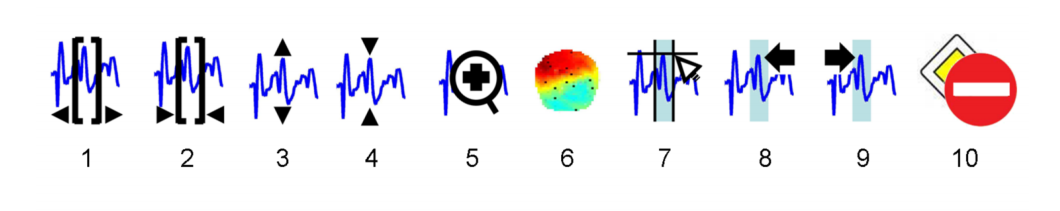
\includegraphics[height=4.5cm,width=15cm]{12.1}
		\caption{SPM M/EEG Review 按钮说明 1-2:增加/减少绘图时间窗口的宽度,
			3-4:增加/减少全局缩放显示因子,
			5:放大,
			7:添加事件,
			8-9:从标记到标记向后/向前滚动数据,
			10:将事件标记为好/坏} \label{fig:12.1}
	\end{figure}



\subsection{脚本生成}

另一种批处理作业的方法是使用 Matlab 编写的脚本。
您可以自动生成这些脚本。
要做到这一点,首先必须使用 GUI 或批处理系统分析一个数据集。
每当调用预处理函数时,所有输入参数在 GUI 组装后都会存储在“历史”中。
通过这个历史,不仅可以详细查看哪些函数被用于数据集,还可以生成重复相同分析步骤的脚本。
主要区别在于,这次不再需要 GUI 交互,因为脚本已经包含了首次运行时提供的所有输入参数。
meeg 对象的历史可以通过 D.history 访问。

要从 SPM MEEG 文件的历史中生成脚本,请在 M/EEG Review 中打开文件并选择 info 标签:此时会显示一个历史标签,显示文件的所有历史。
点击“Save as script”按钮后,系统会询问要保存的 Matlab 脚本的文件名以及要保存的处理步骤列表(默认是全部,但也可以选择其中一部分)。
这将生成一个脚本,运行时会重复相同的分析步骤。
也可以直接调用 spm\_eeg\_history 函数来获得该脚本。

当然,该脚本不仅可以用于重复分析,还可以作为模板用于其他分析。
这些更改只需基本的 Matlab 知识。
例如,您可以替换文件名以预处理不同的受试者,或者更改参数然后重新运行分析。
我们准备了一个示例,使用与上一小节相同的示例数据集来演示这一点(参见文件 man$\backslash$example\_scripts$\backslash$history\_subject1.m)。
通过脚本,您还可以直接使用对象方法,例如添加一行 D=badchannels(D, 23, 1),将通道 23 标记为坏通道(参见过滤步骤后的示例脚本)。
要在您的计算机上运行示例脚本,需要从 SPM 网站下载数据集。